87. Сначала посчитаем, сколько клеток в исходном прямоугольнике: их 39. После это надо приложить букву $P$ всеми возможными способами и посмотреть, сколько клеток она может добавить. При этом надо не забывать, что фигуру можно как поворачивать, так и переворачивать.
\begin{figure}[ht!]
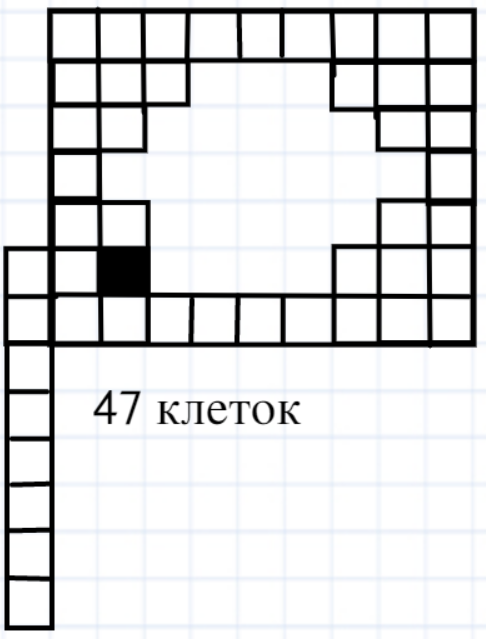
\includegraphics[scale=0.35]{ll1.png} 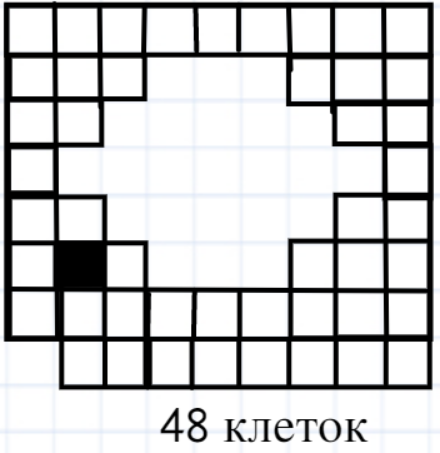
\includegraphics[scale=0.35]{ll2.png}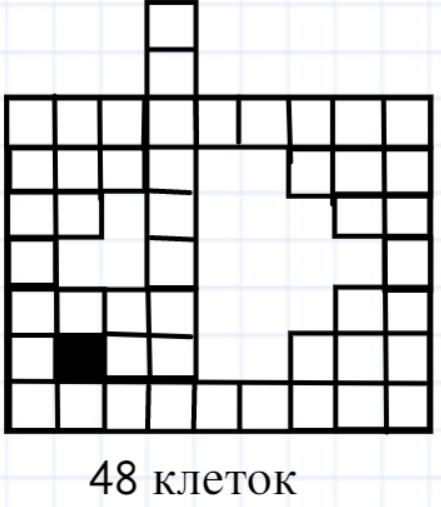
\includegraphics[scale=0.35]{ll3.png}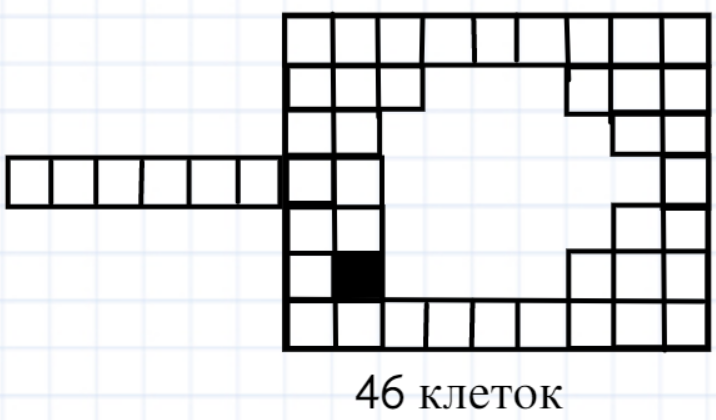
\includegraphics[scale=0.35]{ll4.png}\end{figure}
\begin{figure}[ht!]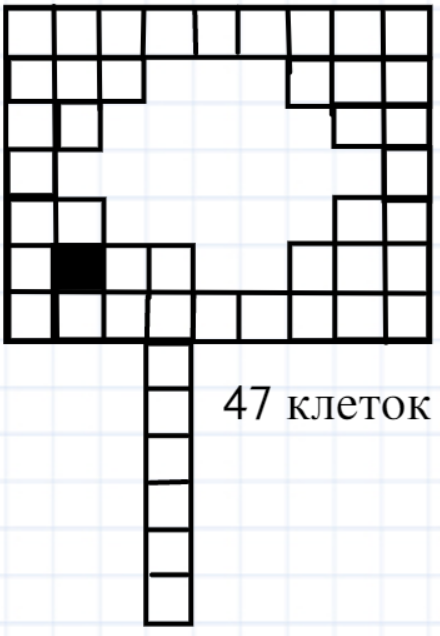
\includegraphics[scale=0.35]{ll5.png} 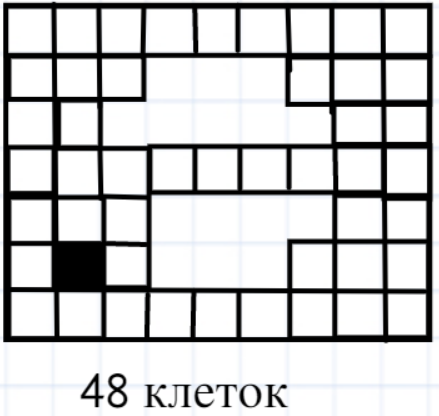
\includegraphics[scale=0.35]{ll6.png}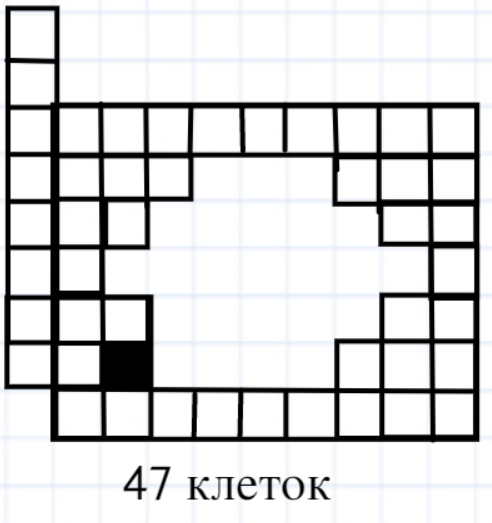
\includegraphics[scale=0.35]{ll7.png}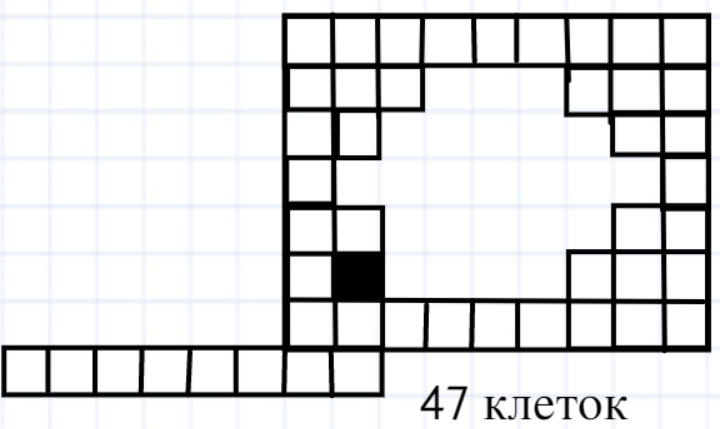
\includegraphics[scale=0.35]{ll8.png}
\end{figure}\\
Как мы видим, возможны всего три варианта: 46, 47 или 48 клеток.\\
